%pdflatex
%%%%%%%%%%%%%%%%%%%%%%%%%%%%%%%%%%%%%%%%%%%%%%%%%%%%%%%%%%%%%%%%%%%%%%%%%%%%%
%
% Vorlage für Seminararbeiten im Institut für Verteilte Systeme
% 
% HINWEISE
% 
%  1. Bei Nutzung für Seminarausarbeitungen darf insbesondere die Schriftart
%     und -größe nicht angepasst werden.
%  2. Die Vorlage unterstützt deutsche und englische Ausarbeitungen durch
%     Anpassung der Klassenoptionen.
%  3. Folgende Angaben sollen angepasst werden:
%     - Titel der Arbeit
%     - Name und E-Mail-Adresse der Autorin/des Autors
%     - Seminar Akronym
%     - Semester
%  4. Die Vorlage sieht eine Lizensierung unter CC-BY-SA vor, die jedoch
%     nicht verpflichtend ist. Falls nicht gewünscht, bitte Copyright auf
%     "retain" setzen.
%     Die gewählte Lizenz (CC-BY-SA) ist kompatibel mit einer möglichen
%     Veröffentlichung auf dem Volltextserver der Uni Ulm
%     (http://vts.uni-ulm.de).
%
%%%%%%%%%%%%%%%%%%%%%%%%%%%%%%%%%%%%%%%%%%%%%%%%%%%%%%%%%%%%%%%%%%%%%%%%%%%%%
%
% Template for seminar papers in the Institute of Distributed Systems
% 
% NOTES
% 
%  1. When used for seminar papers, the font type and size must not be changed.
%  2. The template supports German and English versions by modifying the class
%     options.
%  3. The following information should be adjusted:
%     - Title of the paper
%     - Name and mail address of the author
%     - Seminar Acr.
%     - Semester
%  4. The template forsees licensing under CC-BY-SA, which however is not
%     mandatory. If not desired, please set the copyright to "retain".
%     The selected license (CC-BY-SA) is compatible with a possible
%     publication on the full text server of the Ulm University
%     (http://vts.uni-ulm.de).
%
%%%%%%%%%%%%%%%%%%%%%%%%%%%%%%%%%%%%%%%%%%%%%%%%%%%%%%%%%%%%%%%%%%%%%%%%%%%%%

% Based on the 2017 ACM Master Article Template
% \documentclass[vspaper,language=german]{acmart} % Deutsche Ausarbeitung
\documentclass[vspaper,language=english]{acmart} % Englische Ausarbeitung
\settopmatter{printfolios=true} % Adding Page numbers

% \setcopyright{retain}
% \setcopyright{cc-by}
\setcopyright{cc-by-sa}

%Seminar Akronym = KTT, PRIV, PASF, ATVS oder RTDS
% \acmConference[ATVS]{Ausgewählte Themen in Verteilten Systemen}{WS 2021/22}{Institut für Verteilte Systeme, Universität Ulm}
\acmConference[ATVS]{Seminar Type Long}{WS 2021/22}{Institute of Distributed Systems, Ulm University}


%%%%%%%%%%%%%%%%%%%%%%%%%%%%%%%%%%%%%%%%%%%%%%%%%%%%%%%%%%%%
\usepackage{graphics}
\usepackage{float}
\graphicspath{ {figures/} }


\begin{document}

\title{First Packet Authentication}

\author{Emilija Kastratović}
\email{emilija.kastratovic@uni-ulm.de}

\hbadness=10000
\maketitle
\hbadness=1000



\section{Abstract}
Cybersecurity and secure packet-based communication already start at the very first packet that is sent from one host to another.  The first packet builds the foundation for the following communication, and thus the initiation must be as secure as possible.  First Packet Authentication (FPA) describes a notion of how such security and authentication can take place.  \par
Methods like Port Knocking (PK), Single Packet Authorization (SPA) and BlackRidge Technology's Transport Access Control (TAC) provide such services.  All aim to ensure that the first packet sent is properly authenticated, authorized, and poses no threat to the target system.  This paper will describe and evaluate the methods as mentioned above of First Packet Authentication.\\\par
\section{Introduction}
\label{sec:introduction}

Cybersecurity is becoming more and more critical to any technology nowadays.  Data protection has shifted to become a crucial component of any service, as virtually everything is becoming completely digitalized, thus creating more and more vulnerabilities.\par

Unauthorized access must be made practically impossible to ensure security and deter attacks.  Nevertheless, long before this information is extracted in an attack, the system needs to be breached.  Moreover, basic communication needs to occur between the system and the attacker even before that.  This first step must be as secure as possible, and for it to be ensured, there are many different approaches based on a similar foundation.\\\par

As defined by MODINS, authentication "is the corroboration of a claimed set of attributes or facts with a specified or understood level of confidence" \cite{modins}. \par

It all starts with the first packet sent to the target system.  The target system must not just accept anything that it receives.  A so-called zero trust approach in networking is the basis for that.  The zero trust, also called explicit trust, principle assumes that all network traffic is a threat until authorized, and all traffic needs to be validated.  Explicit trust means that devices should not be trusted by default, even in a supervised and trusted corporate network and even if previously verified.  Unlike implicit trust - "connect first, trust later" - the idea behind this security model is "never trust, always verify".\par

Essential for the zero trust approach to be realized is that even in an unauthorized request, the system must ensure that no information about the system is disclosed.  Thus, no response shall be sent to the requestor at all.  Even a denied TCP connection reveals information about the nature of the network that can be gathered by attackers to later exploit weak points in the system.  However, First Packet Authentication is a mechanism to prevent that any kind of information about the network is disclosed in the first place \cite{7796146}.  The motivation for such an approach is to avoid host discovery.  The network essentially becomes a "black hole", emitting no information of any kind (not even a SYN/ACK packet) until the right to communicate with network resources is established, thus disclosing no information.\\\par

This paper will outline the different approaches and use cases, ensuring that the very first communication between a server and client follows the Authentication principle of cybersecurity.  All of the following methods present the opportunity for First Packet Authentication to take place. Furthermore, it is evaluated whether the schemes resist common types of cyberattacks and if the foundation of the zero trust approach is sufficiently implemented.\\\par

\section{Approaches}
\label{sec:Methods}

The following section will describe the most popular methods of First Packet Authentication and how they work.

\subsection{Port-Knocking}

Port Knocking (PK) is a method used to open ports on a firewall externally and is an application that offers protection by concealment of network ports, countering port scanning, as all ports remain closed \cite{8494695}.  Usually, PK is implemented with a server-side daemon is configured to watch the firewall log for client-side connection attempts; however, it can be also be implemented at kernel level with a kernel-level packet filter \cite{kernel}, or at a higher level application level.  Note that only the packet headers are used for authentication.\\\par
It waits for a specific sequence of packets before granting access to the services behind the firewall.  The packet itself can consist of any number of packets on the transport layer or even other underlying layers and is similar to a secret handshake.  The complexity of the knock can vary immensely. 
After authentication, the firewall is temporarily reconfigured to allow communication between the client and server.  The session is kept alive after an established connection between the client and the service.
PK is stateful.  That means that no further knocking is allowed in the event of any wrong knock.  Since the zero trust approach is implemented, the remote user is not given any information as to which knock was unsuccessful, as no packets are sent to the client at any given time.\par


\subsection{Single Packet Authorization/Authentication}

Understanding Port Knocking is essential to understand Single Packet Authorization (SPA) because it is one of the most popular types of PK.
SPA was invented in the early 2000s and was commonly used for root SSH access to servers \cite{networkinsight}.\\\par

Note that the keyword 'Authorization' in this context is misleading. To explain, authorization is the process of specifying access rights to resources by specific users.  However, when establishing a connection for SSH, for example, the remote user needs to be authenticated, not authorized, and they are doing that with the first and only package sent.  Thus 'Authentication' would be more precise in this method.  However, since 'Authorization' has been widely used for this method, this paper will also resort to 'Authorization' to avoid confusion.\\\par

Similarly to PK, SPA uses a SPA server and SPA client.  However, unlike PK, where any number of knocks (and usually more than one) is used, SPA's idea is to use one encrypted knock for authentication.

The Single Packet Authorization packet has the following structure \cite{SPAwiki}:
\begin{itemize}
    \item 16 bytes of random data, renders the packet unique
    \item local username
    \item local timestamp, preventing replay attacks
    \item FireWall KNock OPerator (fwknop) version
    \item mode (access or command)
    \item desired access (or command string)
    \item MDA5 sum
\end{itemize}

Firewall Knock Operator (fwknop), developed by Michael Rash in the early 2000s \cite{SPAwiki} and is a Linux tool used to implement SPA on a system.  This, and its default configuration, is the implementation that is going to be referred to when talking about SPA.\par

\begin{figure*}[h!]
    \centering
    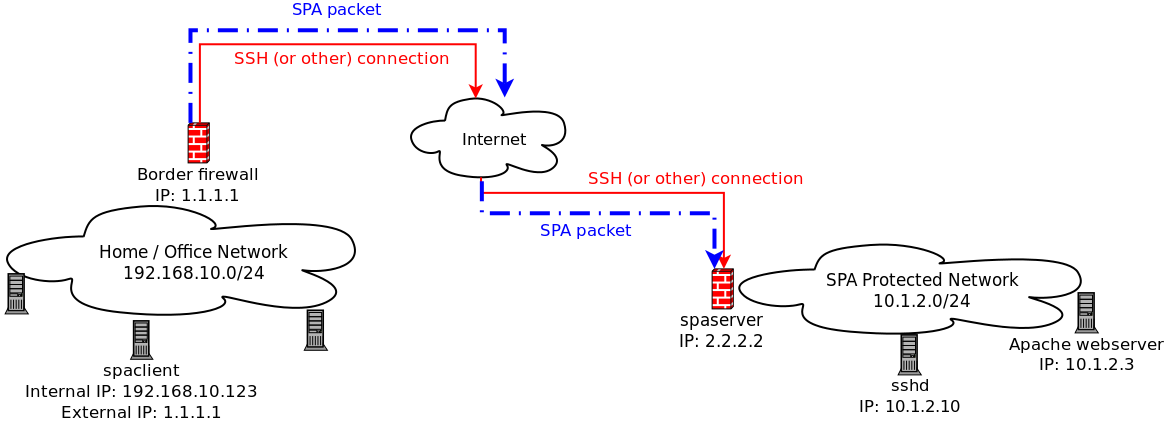
\includegraphics[width=\textwidth]{figures/fwknop_SPA.png}
    \caption{Visualization of SPA using fwknop \cite{spaimage}}
    \label{fig:fwknop_SPA}
\end{figure*}

This payload is encrypted using the MDA5 cryptographic hash function.  The cryptographic key is derived from a password (8-16 characters) entered by the user through a series of the hashing as mentioned earlier algorithm.  This results in approximately 9516 (100-bits) keys \cite{jeanquier}.  Although TCP and ICMP are also possible, SPA did not need to introduce a new protocol but uses UDP to send the authenticating knock.  SPA packets also use the packet payload to communicate authentication information, not just the packet header like PK.  The encrypted authentication data is thus then sent in a UDP packet to the specific server.  The fwknop daemon listens on UDP port 62201 or incoming packets.  When received, the daemon decrypts the data and matches it with the MDA5 checksum.  The daemon also can perform passive fingerprinting of the client and be configured only to allow access to certain machines.\\\par

Similarly to PK, after a successful knock, a connection is established, and the session is kept alive by the 'conntrack' system.  Short for 'connection tracking', conntrack is a system in the Netfilter, which makes up the basis of firewall Linux, allowing the established sessions to remain alive even though the firewall is on the default drop.  IP tables and packet filtering are part of Netfilter in Linux kernels \cite{8494695}.\par


\subsection{First Packet Authentication and Transport Access Control}

The following method to be described was developed by BlackRidge Technology and is named Transport Access Control.  Following the explicit trust principle, Transport Access Control already blocks unauthorized, anonymous traffic at the first packet.\\\par

Like SPA, Transport Access Control did not need to invent a new protocol; instead, it uses the well-established TCP/IP protocol to transmit packages.  TAC is complementary to existing security technologies. Additionally, the size of TCP/IP headers is not increased, enabling Transport Access Control to function without consuming any network bandwidth.
Each network session is authenticated at the transport layer before any access to the target and its services is provided. TAC is thus tolerant of network and port address translation and is designed to operate transparently without introducing its own port or network translation complexity. \\\par 

TAC works on the inside and outside. Externally, TAC protects against unauthorized access, port scans, and network observation.  Internally, TAC prevents viruses, malware, and rogue applications from contaminating adjacent networks \cite{blackridge}.\par

\begin{figure*}[h]
    \centering
    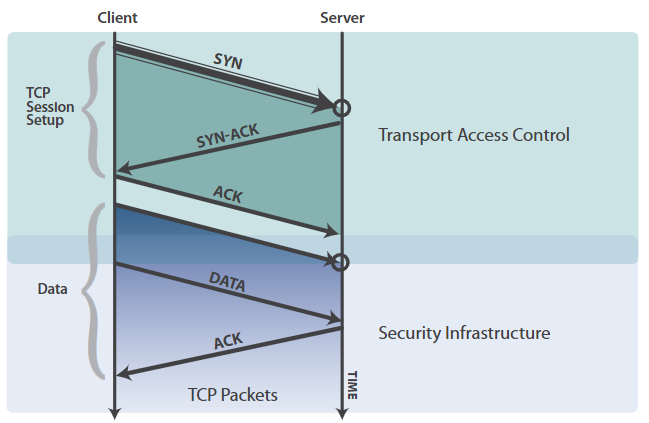
\includegraphics[width=\textwidth]{figures/TAC_arch.png}
    \caption{TCP handshake with TAC (indictated by the SYN packet arrow being framed)  \cite{blackridge}}
    \label{fig:TAC_arch}
\end{figure*}

The first step to authentication is done by generating a network identity token during the session.  This token is a 32-bit encrypted single-use object which expires after four seconds which is generated individually and cannot be reused.  Tokens are associated with identities from already existing Identity Access Management systems and credentials, like Microsoft Active Directory or the one used by Amazon Web Services. In addition, TAC uses an identity token cache to provide high scalability and low latency. \par 
They are generated for each unique entity (typically user or device) requesting access to the network.  Zero trust is established by authenticating said identity tokens and applying a security policy on the first TCP packet before any sessions with network resources can be established.  Next, an in-line virtual security gateway is established between the protected resources and the rest of the network.
Once authenticated, sessions between the server and client can be established.  If authentication fails, unauthorized traffic is rejected from the network, and again, there is no feedback to the client, preventing attackers from gathering any information about the network \cite{blackridge}. \\\par

\begin{figure*}[h]
    \centering
    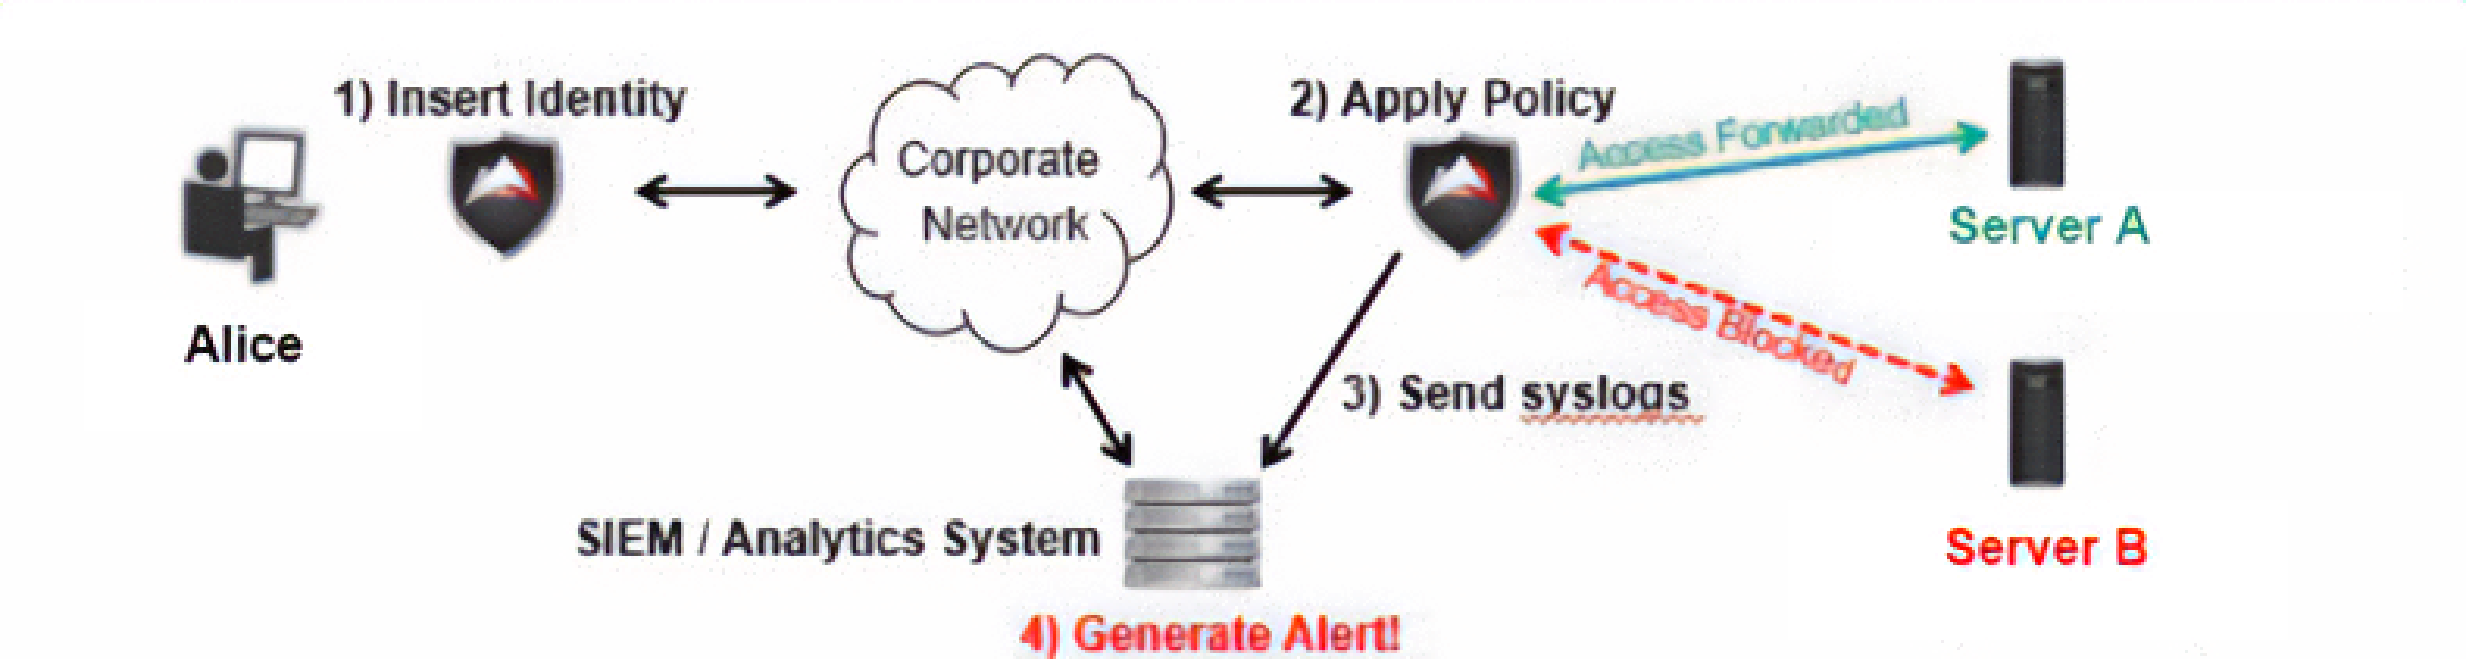
\includegraphics[width=\textwidth]{figures/alice_tac.PNG}
    \caption{TAC token authentication \cite{8494695}}
    \label{fig:alice_tac}
\end{figure*}

Figure ~\ref{fig:alice_tac} illustrates this behavior: Let there be a server A and a server B within the same network, and a user Alice who is authorized to access only server A.  A TAC gateway appliance is connected in the path between Alice and the rest of the network.  Another gateway is positioned before the protected resources.  The first gateway inserts an identity token in the first packet of the TCP connection request.  The second gateway enforces the network access policy by extracting the token, resolving it to an identity, and determining its authorizations.  If Alice attempts a connection request to server A, the gateway grants access and the connection is completed.  However, if Alice is attempting a connection request to server B, the request is denied and discarded, and Alice receives no feedback from the system in case of connection request failure.  The connection attempt is logged, and important to note is that continuous logging of all access attempts is constant with the approach of a zero trust network (i.e. not allowing any access attempts to go unmonitored).\par

When the second gateway receives a connection request, it extracts and authenticates the inserted identity token and, based on the received entity, then applies a security policy (such as forward, redirect, or discard) to the connection request.  This gateway acts as a policy enforcement point that is transparent to the rest of the system architecture. Also, it is backwards compatible with existing network technologies.\par  
If the network access token for a TCP request fails to resolve to an identity or resolves to an identity that lacks the authority to access the requested resource, the connection request is rejected without further response to the requestor.  In this way, the requestor receives no information about what sort of devices might be attacked behind the gateway, effectively cloaking the presence of a protected scientific instrument or data repository \cite{blackridge}.\\\par

In summary, TAC authenticates the first packet of a session, blocks network scans (by cloaking TAC-protected systems from unauthorized users) and filters and controls network access to resources while preserving existing concepts in cybersecurity and provides low, deterministic latency with highly scalable throughput \cite{blackridge}.\par


\section{Evaluation}
\label{sec:eval}

The following section will discuss the advantages and disadvantages of each aforementioned described methods of First Packet Authentication and whether zero trust is present.\par


\subsection{Importance of zero trust}

Before starting with the individual methods, it is crucial to emphasize the advantages all have in common, namely the zero trust system.  Implicit trust stems from an age where once inside physically the network, one authentication suffices.  In our highly digitalized world, which is shifting more and more to cloud technology, the physical location of a system is becoming less and less important.  In most modern enterprises, networks consist more and more of cloud-based services and infrastructure, including connections to mobile and remote hosts, leading to increasing connections to non-conventional IT.  
Thus, it is critical to ensure that only authorized users have access to confidential resources, and zero trust plays a vital role in this approach. The growing cybersecurity threat requires an architectural redesign of networks based on the principles of a zero trust network \cite{7796146}.   \par
Attackers wanting to gain unauthorized access to a network or service can attack anywhere.  However, zero trust disrupts an attacker's strategy of OODA (observe, orient, decide, attack), since with explicit trust, the target is wholly cloaked, and thus no observation can take place.\par


\subsection{Port Knocking as a solid foundation}

%security through obscurity
Port Knocking is a security example that is, in a sense, security through obscurity.  Security through obscurity is a security design in which the principle of how a system works is kept secret.   That is not a wrong design choice; however, relying solely on one principle is the problem.  With this choice, the authentication method itself does not have to be encrypted; nonetheless, it must not be known what the actual method is.  PK is not just another plain text password - at least when used to protect services that listen on a TCP port like SSH.  This makes it more difficult for attack because they will have significant problems breaching the system regardless of their skill level if they know everything except the actual entry point/way to a system.  An attacker will eventually resort to a brute force attack.

%brute force
Thankfully, PK stands strong against brute force attacks.  The average case for a three-port knock requires approximately 141 trillion (65535\textsuperscript{3} / 2) \cite{portwiki} packets to determine the uninterrupted correct sequence.  In combination with limiting knock-attempts, longer and/or more complex sequences and cryptographic hashes, successful port access attempts are challenging.\\\par

%concealment of ports
The concealment of ports is a significant advantage of PK.  Port scanning by a possible attacker is impossible, and no open ports mean no entry into the system.  PK implies that service discovery with tools like Nmap is no longer possible.  The only way in is knowing the correct sequence and types of knocks.  However, this also presents a major disadvantage.  PK is secure until the secret knocks are known.  Once that information is out, and assuming that the information gets into the intent of malice, this security mechanism becomes void, and the system can be breached.\par
Nevertheless, even with all the possible solutions mentioned to make PK secure, the main problem that no paper has mentioned is that it first needs to be transferred over a secure channel for the requesting party to know the knock sequence.  Neither PK nor SPA are a solution for this; yet, this is the first step in the process.  Without knowing the correct knock sequence, DoS takes place for any user.\\\par

%out of order
The Internet is known for various latencies.  Although basic PK might work flawlessly in a local network, the delays in network communication occurring over larger areas suggest a problem when attempting to use the mechanism in practice.
It cannot be ensured that the packets arrive in order; thus, PK suffers from out-of-order packet delivery.  Latency can result in a rearrangement of packets, and weak Internet connections can lead to packet loss. As previously described, any wrong packet will render all the previous and next packets useless, and PK needs to be performed again.  Time delays for each packet might resolve this issue while also slowing the whole process down \cite{PKissues}.  Broadcast or live streaming activities where a fast transmission of packets and no connection between both parties needs to be established is inconvenient with this method.\par
The question of what happens in the case of two users knocking at once must not be overlooked.  The stateful behavior of PK is a smart design choice, as it allows several users from different source IP addresses to be at different stages of PK simultaneously.  This way, the PK daemon can differentiate between knocking clients and authorize each one in turn as the correct knock sequence is received.  This allows a legitimate user that used the correct knock sequence to pass the firewall while the firewall itself is in the middle of port knocks from multiple IP addresses.  From any other IP address, the ports on the firewall will still appear to be closed.  This solves a possible DoS for the users, as each would break the sequence of one another.\\\par

%mitm
Another flaw of PK is that it suffers from attack methods such as man-in-the-middle.  Since the packets are sent in 'clear-text', eavesdropping becomes an obvious exploit.  The correct sequence of knocks can be obtained through packet-sniffing, and performing a replay attack will grant the connection \cite{sushant}. Using cryptographic hashes inside the port knock sequence is a possible solution.  \par
While with PK, it is assumed that the server is secure, the client is known to be a weak point, i.e., if the client is compromised, an attacker can exploit an established connection, and PK offers no protection against that.

%client IP spoofing
Additionally, IP address spoofing of the client is a possible exploit and will result in a DoS for the spoofed user.  Especially hosts with a static IP address are vulnerable to this.\par

%robust knocking daemon
PK is also very reliant on the robustness of the port knocking daemon. The daemon can be an undesirable single point of failure.  Failure of the daemon can deny any access - even legitimate and authenticated users - to the system.  The availability aspect of the CIA security principle becomes void.  Implementations use a monitoring daemon that restarts the failed PK daemon - however, this only delegates the problem and do not resolve the issue.  If the monitoring daemon fails, so does this solution.\par

%brute force
Although rarely implemented, deployed PK results in a significant reduction in the amount of bandwidth consumed by SSH or brute-force attack because a possible attacker is forced to be less stealthy, as 'loud' and repeated knocks are more noticeable in network logging \cite{PKissues}.\\\par


In summary, PK offers a good foundation for FPA; however, it lacks the vital encryption needed to prevent the most common cyberattacks. \par


\subsection{Single Packet Authorization enhances Port Knocking with downsides}


Many of those issues require a solution, and those vulnerabilities were the primary motivators for the development of Single Packet Authorization.  \par
SPA solves most of the problems Port Knocking proposes while retaining all of the benefits Port Knocking offers. Similarly to PK, SPA also follows the zero trust principle in which no information about the system must be disclosed. This alone is, again, a crucial benefit of using SPA.\\\par

Starting with the most notable difference between PK and SPA is that the latter only uses one packet. Subsequently, SPA does not have the issue of out-of-order delivery of packets, as only one packet is needed in the authentication process. However, a single knock over a few has its downside, too. Detecting SPA packets is more difficult than detecting port knocks as SPA packets are less obvious than long and repeated port knocks and contain seemingly random data which can potentially blend in with normal network traffic. However, using fwknop, some indicators could be added to an Intrusion Detection System (IDS) to note that fwknop is in use on the network.  Fwknop packets, by default, go to port 62201, so a rule could be defined to watch for traffic to that port, although this would easily be bypassed by switching to a custom port \cite{jeanquier}.  Alternatively, an IDS can attempt to track fwknop packets by checking the data length of the UDP packets.  A fwknop packet encrypted using AES encryption is 80 to 160 bytes in length.\par
Nevertheless, for example, a packet encrypted using GPG is between 500 and 1600 bytes in length.  Thus, this proposes a possible solution to track SPA packets. An additional advantage over PK is that replay attacks that are possible are now impossible to execute since the payload includes a timestamp.\\\par

Another enhancement SPA offers over PK is the usage of cryptography. PK, as described, are sent in 'plain text' with no encryption or payload. On the other hand, SPA makes intelligent use of the payload and encrypts it additionally. By encrypting the authentication string that contains a hash of the data, the plain text becomes integrity-protected, and thus an attacker would be unable to change the plaintext (through ciphertext manipulation) without those changes being detected.  \par 
Encryption is crucial in today's security, but it comes with much overhead. Essential to understand is that fwknop uses a user-given passphrase in order to hash and encrypt the payload. By default, this renders fwknop to be especially vulnerable to dictionary or brute force attacks. An attacker could intercept the authorization packet and perform a dictionary attack by testing a list of possible passwords and comparing the values.  If the two hash values match, the correct password has been found.  This, in return, requires knowledge of a possible username authorized on the target system. However, since 'root' is a common user, in fact, the 'superuser' or 'administrator', on every Linux machine, unauthorized root access is not too challenging to achieve.  The timestamp needed can be obtained by looking at the computer clock when the packet was intercepted,  and the IP address can be spoofed or recovered from the IP header of the user's UDP packet.   If any dictionary attack is successful, the attacker could authenticate themselves and, e.g. instruct the server to open any port for later access, with no authentication needing to occur; essentially, the system is completely breached. Fwknop can be modified to support any length for passphrases, which would allow users to use long passphrases, significantly reducing the threat of dictionary attacks.  Although this greatly reduces the threat of dictionary attack, a memorable passphrase would have to be 39 characters long before it was of similar strength to an AES 256-bit key \cite{jeanquier}.\par

Security of SPA solely relies on the encryption method used. The hashing algorithm MDA5 sufficed when fwknop and SPA were invented; however, it has evolved to a well-known deprecated and insecure algorithm. In addition, the main drawback to fwknop is that encryption is achieved by using symmetric encryption. This can be solved by using asymmetric cryptography.  Each user has their own private key, which can be used to sign the authorization data when the data is encrypted with the server's public key.  It is trivial to transmit information securely to the server without resorting to the brute-force method involved with symmetric keys.\par

Man-in-the-middle is once again an issue. Since the target IP address lies unencrypted in the UDP header of the packet, it is very easy for the attacker to intercept an authentication packet, change the IP address to insert their own IP address. The result is that the attacker obtains a free pass to the target system, as the IP address is not included in the encryption process. With fwknop, it is possible to grant access to any IP address, and in return, no spoofing would be needed again.  \par
Similarly, an IP spoofing attack can be performed and obtaining an IP address from an authorized user would result in the same attack as mentioned above.\\\par

Another critical issue that both PK and SPA share is the vulnerability of the user. A compromised user renders even the strongest and most layered security mechanisms useless. Without security on every level and at every node, no security is possible. A major downside to all of the discussed methods of securing a system never emphasizes the user. PK, SPA, and TCA surely help create a 'black hole' for any outsider but offers no protection against successfully authenticated and authorized users. All of the approaches ignore the fact that once inside a system, authentication needs to occur. zero trust is only established at the most outer layer by choosing to authorize the first interaction with a system sufficiently. Nevertheless, zero trust needs to be implemented at every given layer to a resource.\\\par

To summarize, SPA offers major advantages over PK while retaining all of the benefits. The inclusion of encryption and a single packet are the key differences in why SPA is superior to PK. However, it heavily relies on the fwknop configuration and encryption strength and offers no zero trust protection once inside the network.\par



\subsection{BlackRidge Technology's Transport Access Control improves TCP}

A subject with TCP does not exchange identity credentials until after a session is fully established.  This design exposes confidential resources to attack.  One can not know whom the network is exchanging information with until the conversation is underway.\par 

Transport Access Control improves TCP and proposes a solution to this vulnerability using cryptographic identity tokens to authenticate TCP requests before the session is fully established.  No exchange takes place unless the requestor displays a pre-determined shared secret.  This is a massive difference between PK and SPA. Whereas the two schemes use existing standards like TCP or UDP, TAC takes the well-established TCP and improves upon it. \\\par 

TAC shares the same advantage as SPA, as the authentication process takes place with one packet, unlike the many loud packets sent by PK. This makes TAC faster and more efficient, as the same result is achieved in one step. The aforementioned token cache is tolerant of packet loss and enables TAC deployments in low bandwidth and high packet loss environments. This eliminates the problem of out-of-order packet delivery that PK features. Note that TAC is a newer approach to PK and SPA. The algorithms used in TAC are highly parallelizable. This enables high scalability to take advantage of today's multi-core and multi-processor systems.\\\par

TAC clients and policy engines can be hosted on a wide variety of platforms.  It works for any network topology or addressing scheme, like IPv4, IPv6, and networks that use the Network Address Translation (NAT) protocol. It is also compatible with dynamic addressing often used with mobile devices. This approach has several advantages, including separation of security policy from the network design (addresses and topologies) \cite{blackridge}. This approach extracts, authenticates, and applies policy to the connection requests. This protects against unauthorized external observation of the network devices and stops any malware within the protected devices.  Zero trust within the devices is a feature that both PK and SPA lack, so this is a significant bonus point for TAC.\par
Security policies can be easily applied to conceal network attacked devices from unauthorized awareness at the earliest possible time.  TAC blocks both known and unknown attack vectors by preventing unauthorized awareness and access.  This approach is high bandwidth and low latency since packet content is not inspected. Network Tokens do not consume otherwise valuable data bandwidth,  as they are embedded in the TCP session request. The combination of TAC and a segmented, multi-tenant network implements a layered defence against cybersecurity threats and contributes to the non-repudiation of data.
These techniques are also well suited to protecting cloud resources such as enterprise-class mainframe computers.  Further, this approach can be applied to protecting the centralized SDN network controller from unauthorized access and enable only authorized SDN controllers to manage and configure the underlying network \cite{blackridge}. \par
TAC is also a more approachable implementation for home networks, where knowledge of handling fwknop is not needed. This is a more passive approach to security than is the case with the approaches mentioned earlier. This way, TAC cloaks and subsequently protects network information such as servers from network disclosure, establishing the zero trust principle. As with all three methods, port scanning is impossible, and a powerful tool like Nmap is rendered useless. TAC works with all TCP based applications and is compatible with existing networking and security infrastructure \cite{blackridge}.\\\par

The most significant weak point of TAC is the considerable reliance on the token used to authenticate an authorized user and proposes several vulnerabilities.\par
First, using a third-party Identity Access Management (IAM) ; compromise on that behalf would break the whole system, as the vital identity token cannot be obtained to complete authentication. Second, an attacker can impersonate the user and complete authentication by spoofing or token sniffing if an attacker gets a valid token. Nevertheless, a token brings benefits, such as that the token prevents replay attacks, as the token is usable only once and expires after a few seconds. In conclusion, the token generation and insertion must be ensured to be secure. \par

To put it briefly, TAC is an approach that differs a lot from Port Knocking implementations. It improves the already existing TCP, unlike the PK schemes that solely rely on it. It is easily implemented in existing infrastructure with no additional overhead. Furthermore, it retains benefits of an external zero trust like the other approaches and extends them to the inside.\\\par

\section{Conclusion}
\label{sec:conclusion}

Cybersecurity is a highly complex and layered topic.  Each of the discussed techniques is a way to secure and protect data, and every method has its advantages and disadvantages.  \par

Even though the technologies mentioned earlier have not evolved to become the conventional approach to security, their foundation on explicit trust rather than implicit trust is an approach that should be established more often and become the norm in today's highly digitalized world.  \par
It is essential to note that there is no one method to secure a system; every system has its vulnerabilities. Each component that plays a role in security needs to be as strong and unreachable as possible, for the security is dependent on its weakest link.  It always depends on the security architecture, the security experts, and the people who use cybersecurity methods to state which approach shall be used for what purpose to ensure that no malice finds its way into a system.\\\par 

Port Knocking has shown to be a good foundation for the later and improved-on Single Packet Authorization (or better: 'Authentication'). However, Single Packet Authorization fell short as the current most popular implementation depends on a single tool that, as or right now, is not part of the standard Linux kernel.\par

BlackRidge Technology's First Packet Authentication, with the help of their Transport Access Control, improves the already existing TCP protocol and can even be expanded to other technologies. It shows that an already well-established system has the potential to improve and make this zero trust approach the new standard for TCP.\par

Although TAC provides security within the system, unlike Port Knocking and Single Packet Authorization, none of the approaches provides protection to the user initiating a connection to the secured system. Zero trust needs to take place at all levels. Nevertheless, these mechanisms offer a step in the right direction.\\\par

In conclusion, a layered approach resulting with defence in depth and security through obscurity, in combination with the zero trust security design, proposes a solid strategy in cybersecurity.\\\par


\appendix
\hbadness=10000
\bibliographystyle{ACM-Reference-Format}
\bibliography{references}
\hbadness=1000
\end{document}
